\documentclass[a4paper, 11pt]{article}
\usepackage{amsmath}
\usepackage{amssymb}
\usepackage[T1]{fontenc}
\usepackage[utf8x]{inputenc}
\usepackage{lmodern}
\usepackage{graphicx}
\graphicspath{ {./images/} }
\usepackage[english]{babel} 
\usepackage{natbib}
\usepackage{cite}
\usepackage[parfill]{parskip}
\usepackage{enumerate}
\usepackage{float}%for image positions
\usepackage{hyperref}
\hypersetup{
  colorlinks,
  citecolor=black,
  filecolor=black,
  linkcolor=black,
  urlcolor=black
}
\usepackage{amsthm}
\newtheorem{theorem}{Theorem}[section]
\newtheorem{lemma}[theorem]{Lemma}
\newtheorem{proposition}[theorem]{Proposition}
\newtheorem{axiom}[theorem]{Axiom}
\newtheorem{invariant}[theorem]{Invariant}
\newtheorem{breakpoint}[theorem]{Breakpoint}
\newtheorem{problem}{Problem}
\newtheorem{definition}{Definition} 
\usepackage{algorithm}
\usepackage{algpseudocode}
\usepackage{pifont}
\usepackage{multirow,array}
\usepackage{centernot}
\usepackage{listings}
\usepackage{xcolor}

\lstdefinestyle{base}{
  language=C,
  emptylines=1,
  breaklines=true,
  basicstyle=\ttfamily\color{black},
  moredelim=**[is][\color{red}]{@}{@},
}

\usepackage{comment} % enables the use of multi-line comments (\ifx \fi) 
\usepackage{lipsum} %This package just generates Lorem Ipsum filler text. 
\usepackage{fullpage} % changes the margin

\begin{document}
\noindent
\large\textbf{Homework 1} \hfill \textbf{Kim Hammar} \\
\normalsize ID2208 \hfill Due Date: 31 January 2017 \\
Programming Web-Services \hfill \\

\section*{Problem Statement}
The given task was to simulate an Employment Service Company that creates application profiles for job seekers. The profiles are XML-based and are produced by extracting data from multiple other sources, including Universities, Employment Officies, Online Company Services, and the user itself.

The task comprise of designing five different XML schemas from different business domains, producing sample documents and performing XML processing. For practice-purpose the XML processing was required to use four different techniques: Document Object Model (DOM)-parsing, Simple API for XML (SAX)-parsing, Java Architecture for XML Binding (JAXB)-parsing, XQuery for extracting information,  and Extensible Stylesheet Language Transformations (XSLT) for transforming XML documents. 
\section*{Main problems and solutions}
\begin{itemize}
\item \textit{Create XML Schemas and generate sample documents.}
  
  The main challenge here was to ensure to be consistent in the design across the different schemas and to follow best pracices.
\item \textit{Parse XML Schemas.}
  
  The tooling support for XML in Java is very flexible and easy to use, one just need to be aware how the libraries differ in the the parsing-paradigms they use.
\item \textit{Extracting information from XML documents and creating new documents}
  
  To automate the process of creating Application-profiles, it is neccessary to parse and extract information from the input XML documents and use the extracted information to create the new XML document.
\end{itemize}
\subsection*{Designing XML Schemas}
When designing the XML schemas I used the following practices:
\begin{itemize}
\item No mixed content in elements, elements either have textual content or child-elements.
\item Only make types or elements global if they are to be reused in some context, otherwise stick to anonymous types.
\item Avoid redundance, reuse when possible.
\item Explicitly use targetNamespace in schemas to make it clear what type of XML documents it is intended to validate.
\item Use child-elements for all type of data that has structure, only use attributes for data that can be considered ``metadata'' for the data in child-elements.
\item Constrain types as much as possible to enforce strict XML documents that is easy to parse and validate.
\item Always use namespaces and qualified names to avoid confusion, e.g impose qualified names for  both local and global elements by  adding: \texttt{elementFormDefault="qualified"} to the schema. To avoid very verbose documents, use default namespaces, as advised in the coursebook:
  \begin{quote}
    \textit{Adding a prefix to every element in the document decreases readability and increases document size. Therefore, XML Namespaces lets you use a default namespace in a document.
    Elements belonging to the default namespace don't require prefixes.} Page 48, \citep{coursebook}
  \end{quote}
\end{itemize}

Apart from following best practices, the main importance when designing the schema was to remember to add linking between courses and degrees in the transcript XML document.
This is necessary to later be able to calculate GPA's for the degrees but still allow flexibility that courses can be in the transcript without belonging to a degree.
I used \textit{Key/Keyref} mechanisms available in XML schema standard to do this, Key/Keyref is very similar to the notion of primary/foreign keys in relational databases, the listings below
show how they were used.

\lstset{language=XML}
\begin{lstlisting}[frame=single,style=base]
  <!-- Each degree should have a unique id -->
  <xsd:@key name="degreeId"@>
  <xsd:selector xpath="./Degrees/Degree"/>
  <xsd:field xpath="@degreeId"/>
  </xsd:key>

  <xsd:attribute name="degreeId" type="xsd:string" use="required"/>

  <!-- A course can optionally be part of a degree -->
  <xsd:@keyref name="degreeIdRef"@ refer="degreeId">
  <xsd:selector xpath="./Courses/Course"/>
  <xsd:field xpath="@degree"/>
  </xsd:keyref>

  <xsd:attribute name="degree" type="xsd:string" use="optional"/>
\end{lstlisting}
A course in the sample transcript XML document can then be linked to a degree as follows:
\begin{lstlisting}[frame=single,style=base]
  <Course @degree="TSEDM-HT16"@>
            <Name>Grid Computing</Name>
            <Code>IJ2208</Code>
            <Credits>7.5</Credits>
            <Date>2016-03-16</Date>
            <Grade>5</Grade>
  </Course>
\end{lstlisting}
This also gives nice flexibility since transcript can easily include courses that is not part of any degree.
\subsection*{Parsing and Transforming}
For \textbf{Task 2} I used SAX, DOM, JAXB, XSLT in conjunction to parse the XML documents and produce the final \textit{application\_profile.xml}. An intermediary step was used where each document was unmarshalled by the different parsing-libraries into in-memory java-structures, before finally extracting relevant information into \texttt{ApplicationProfile.java} and marshalling into XML format.
\begin{figure}[H]
  \begin{center}
    \scalebox{0.47}{
      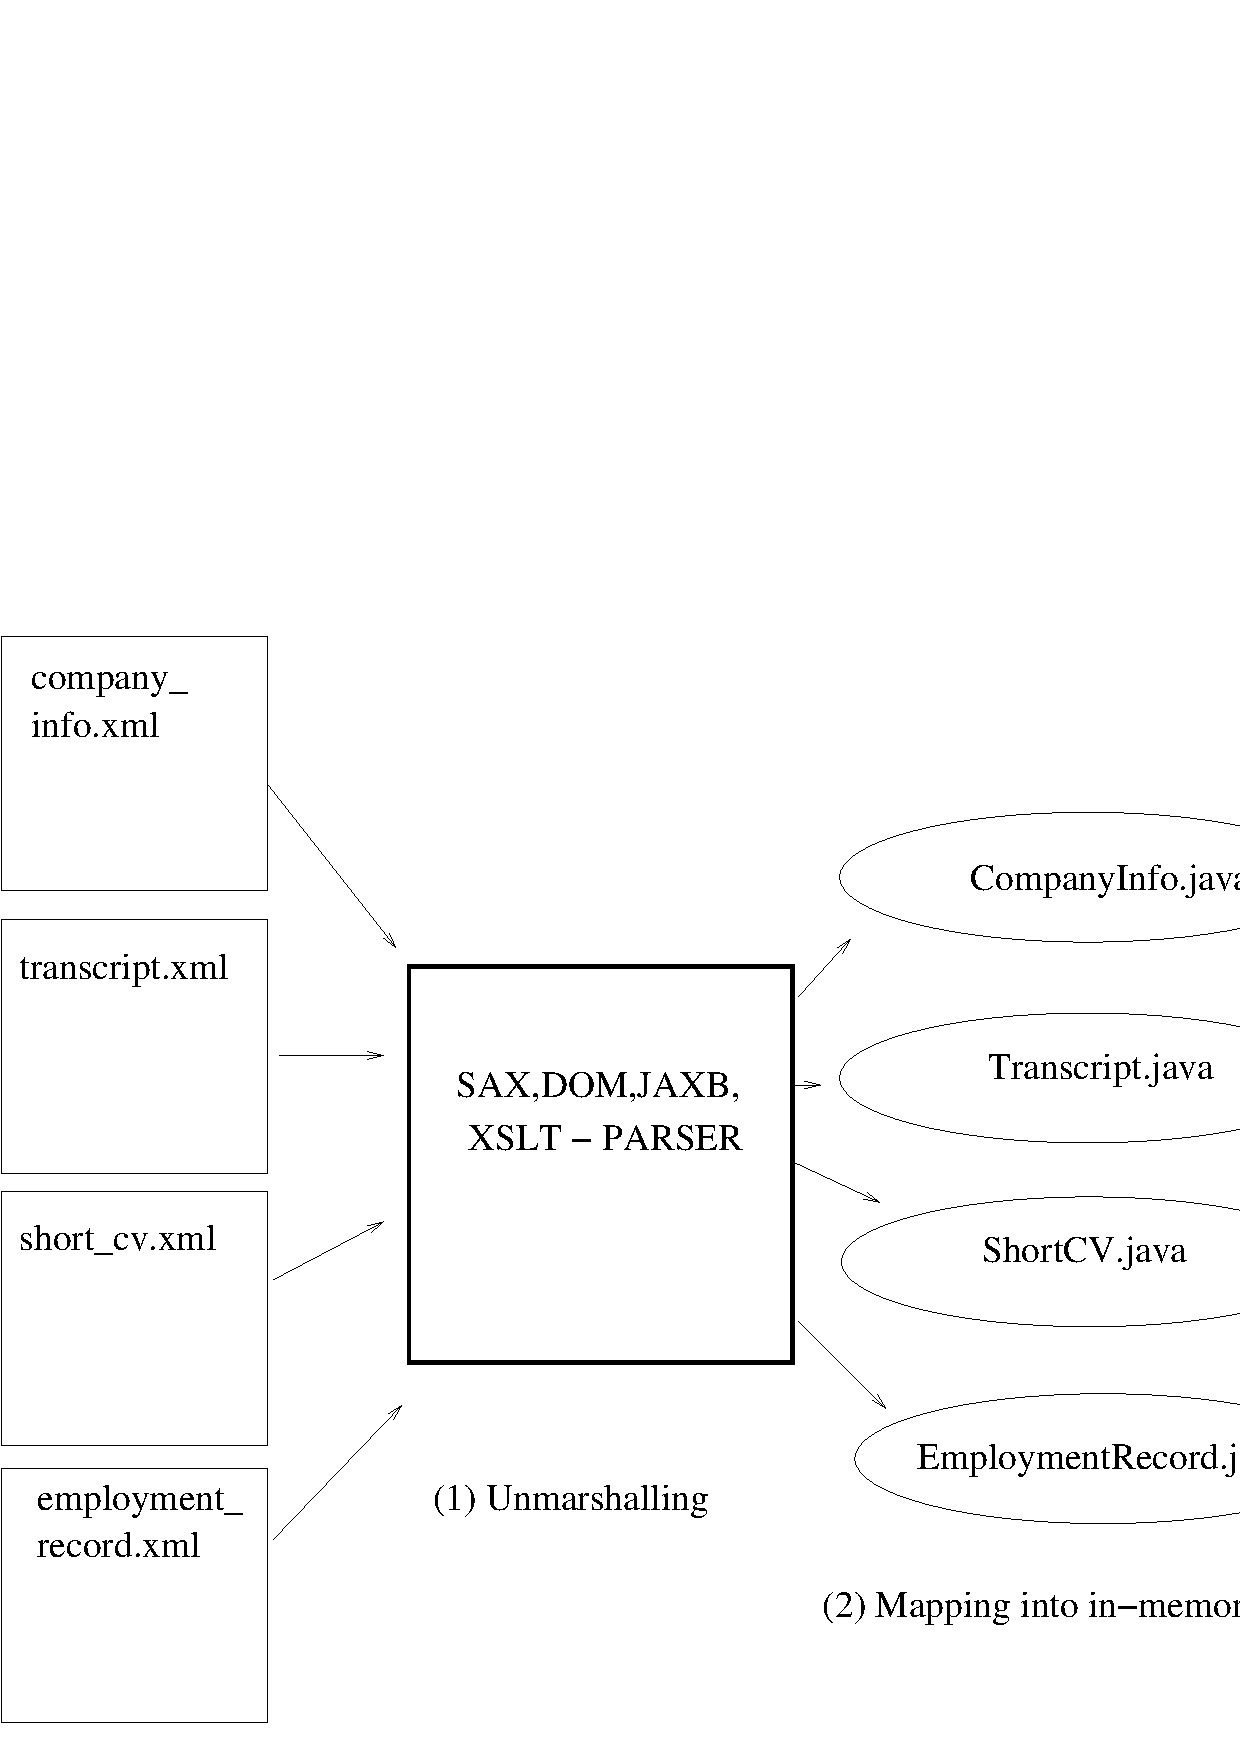
\includegraphics{fig1.pdf}
    }
    \caption{Parsing/Transformation procedure for Task 1}
    \label{fig:fig1}
  \end{center}
\end{figure}
For \textbf{Task 3} I used only XSLT to parse and transform the XML documents and producing the final \textit{application\_profile.xml}. I used an intermediary step here as well, this was preferred over using one single stylesheet due to improved modularity and extensibility.
\begin{figure}[H]
  \begin{center}
    \scalebox{0.47}{
      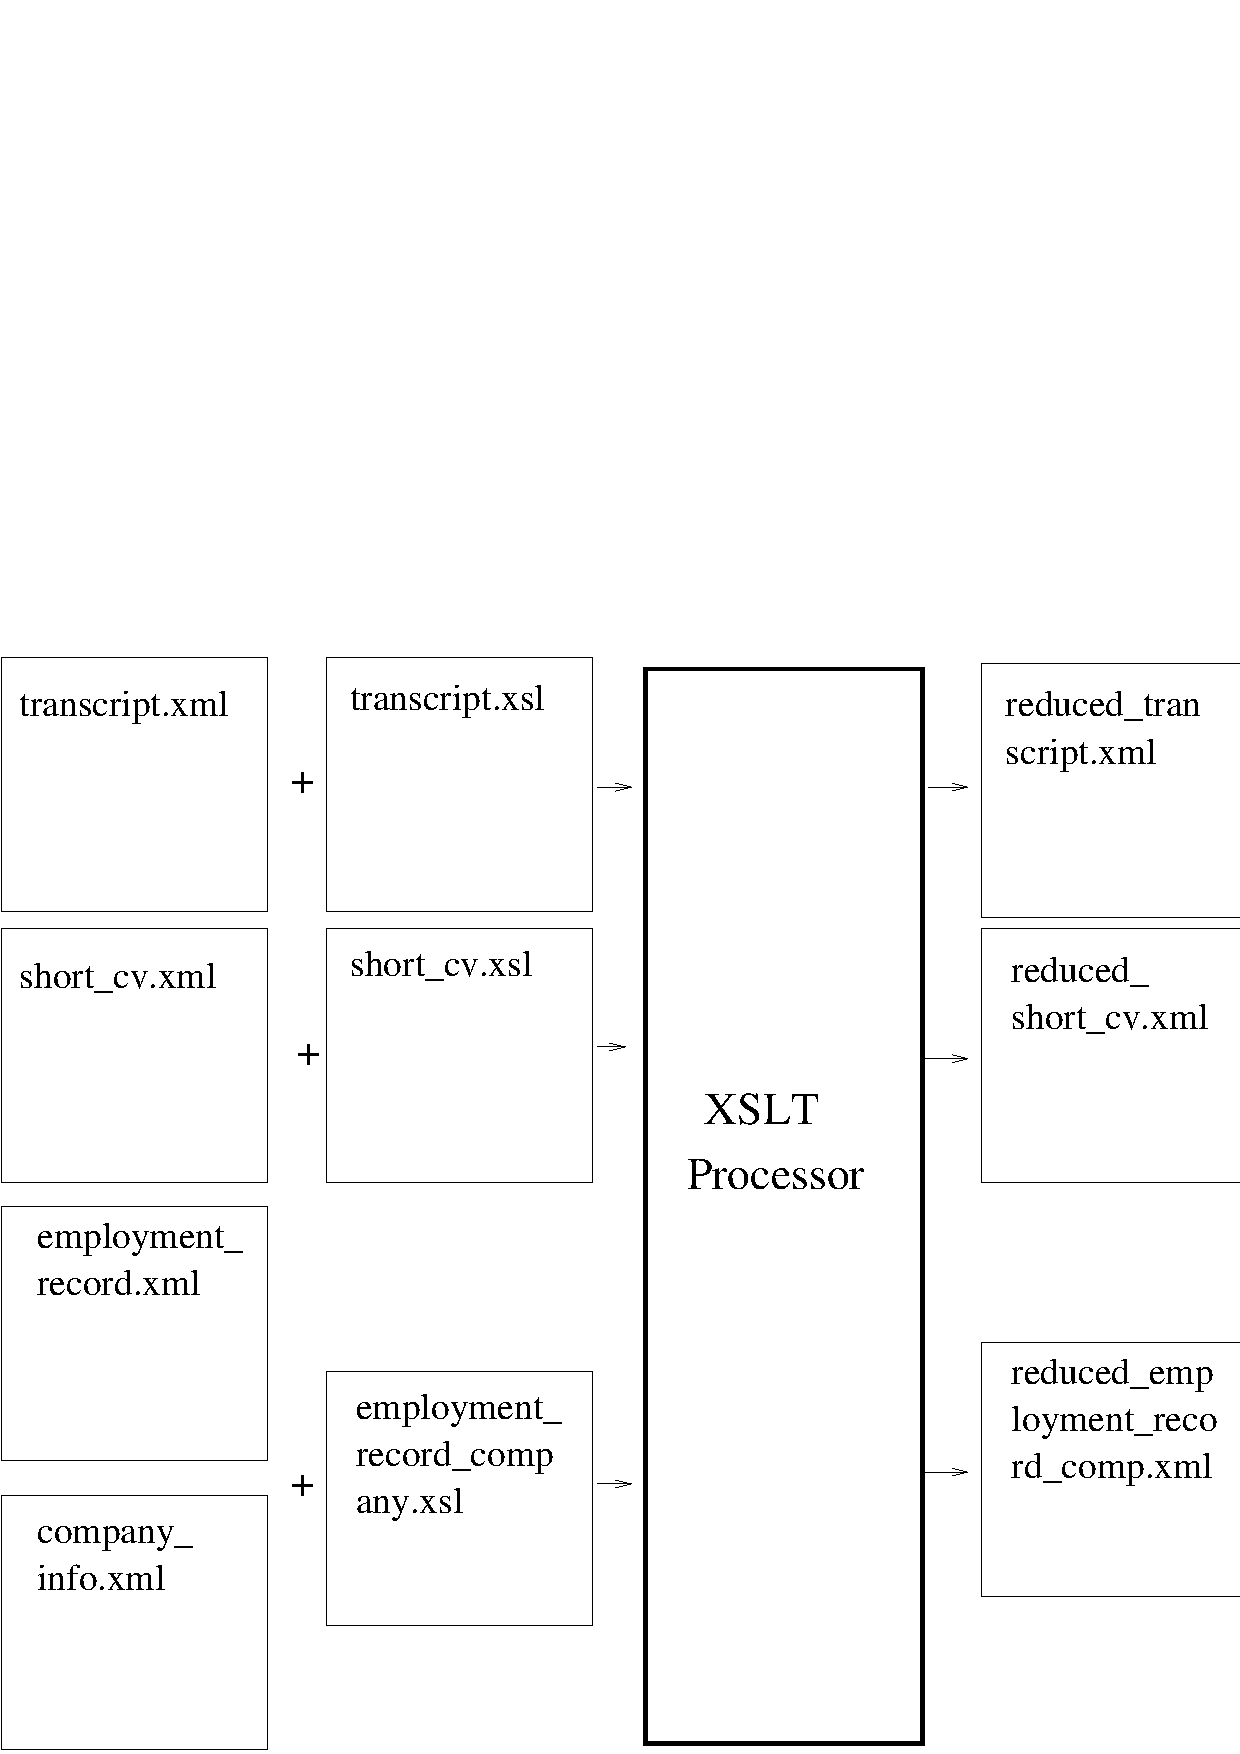
\includegraphics{fig2.pdf}
    }
    \caption{Parsing/Transformation  procedure for Task 2}
    \label{fig:fig2}
  \end{center}
\end{figure}

\section*{Conclusions}
Tooling support for working with XML nowadays is excellent, not least in Java. You have alot of options when working with XML and the best tool/library to use depends on the situation. It is good to be aquainted with the different possibilities to be able to choose the best tool for the job.

\section*{Attachments}
Documented source code can be found in the attached zipfile. See README.MD in the root directory for instructions how to execute and build the program.

\bibliography{references}{}
\bibliographystyle{plain}
\end{document}